\chapter{Aplicaciones}
\label{cap:aplicaciones}

En este capítulo se enumeran y describen las aplicaciones que usarán el mapa que construimos dinamicamente. Estas aplicaciones serán, principalmente, el nodo de localización y el nodo de navegación.

\section{AMCL}
\label{sec:amcl}
\textit{AMCL}\footnote{http://wiki.ros.org/amcl} es un paquete de localización que implementa un algoritmo de Monte Carlo, el cual usa un filtro de partículas para localizar al robot sobre un mapa que previamente le proporcionamos.
\subsubsection{Filtro de partículas}
El algoritmo del filtro de partículas se divide en 4 etapas: Inicialización, actualización, estimación y predicción. 
En la etapa de inicialización se ``lanzan'' una serie de partículas cercanas a la posición inicial del robot. Estas partículas ademas de una posición en el espacio tambien tendrán una dirección. Podemos ver un ejemplo gráfico en la imagen \ref{fig:initamcl}

\begin{figure}[hbtp]
  \begin{center}
    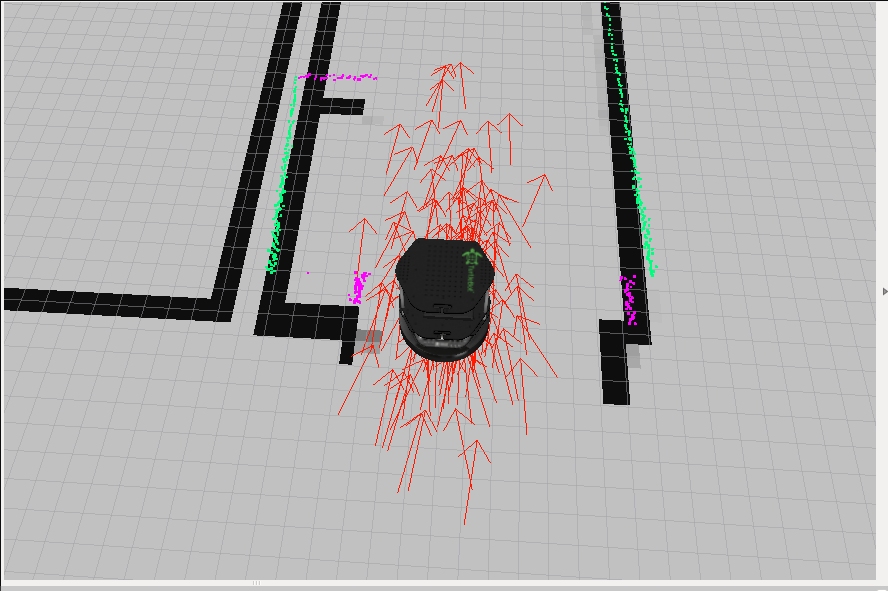
\includegraphics[width=10cm,height=7cm]{img/cap5/initamcl}
  \end{center}
  \caption{Inicialización del filtro de partículas}
  \label{fig:initamcl}
\end{figure}
Vemos como se han generado muchas partículas alrededor del robot y que cada una tiene una dirección más o menos acertada con la dirección del robot.

En este punto del algoritmo se compara la percepción del laser del robot en el punto en el que se encuentra con la percepción que tendria si tuviera la posición y la dirección de cada una de las partículas que generamos. Cuanto más acertada sea la suposición anterior, más valor se le dá a esa partícula. Asi nos encontraremos que las partículas que estan más cercanas a la posición del robot cobran más valor y las que están más lejos y con una dirección totalmente erronea tienen menos valor. Esta fase es la llamada de Actualización. 

En la siguiente fase, llamada de Estimación, nos quedamos con las partículas que más valor tenian para volver a lanzarlas en la siguiente fase del algoritmo.

En la ultima fase, fase de Precicción, lanzamos las partículas de nuevo con el valor que tenian y su posición, añadiendole un pequeño ruido.
En este punto del algortimo tambien se corrige la posición del robot a la posición de la partícula con más valor.
Una vez completado el algoritmo se vuelve a la fase de Actualización y se repite hasta que el robot esté perfectamente localizado en el 
mapa.

\begin{figure}[hbtp]
  \begin{center}
    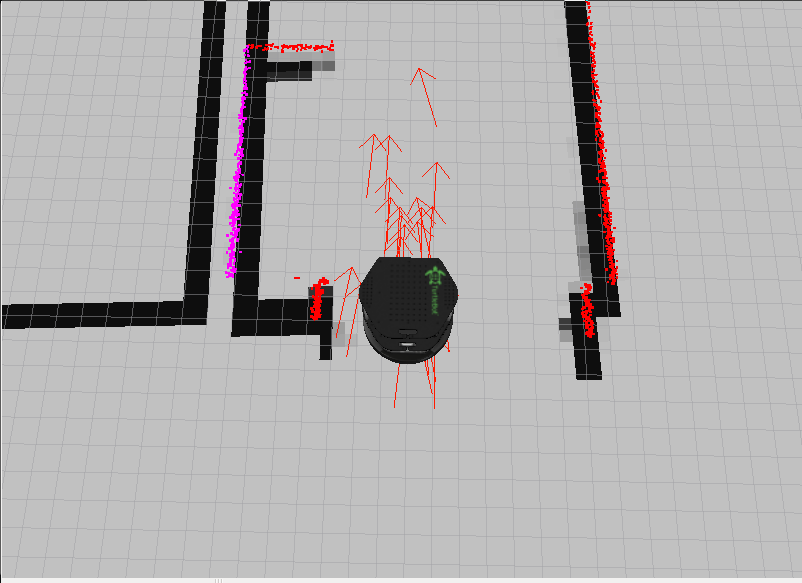
\includegraphics[width=10cm,height=7cm]{img/cap5/actamcl}
  \end{center}
  \caption{El robot se vá acercando a la posición ideal}
  \label{fig:actamcl}
\end{figure}
\pagebreak

Observamos como la linea color de la parte derecha de la imagen \ref{fig:actamcl}, correspondiente a las muestras tomadas con el laser, está más cerca de la linea del mapa que en la imagen \ref{fig:initamcl} que se aprecia que no está alineada. Esto es fruto de la corrección que se va haciendo de la posición. Tambien observamos que hay menos partículas, esto es fruto de la convergencia hacia la posición correcta.

\begin{figure}[hbtp]
  \begin{center}
    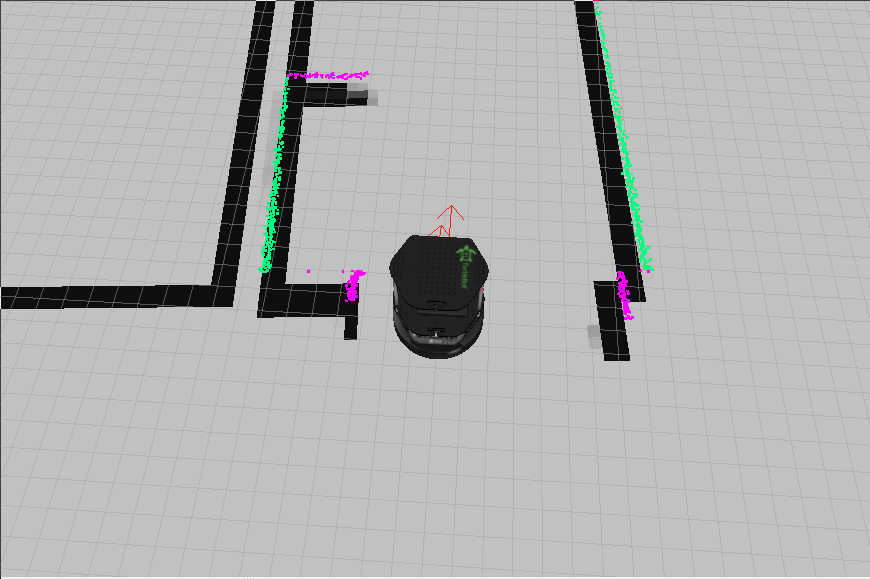
\includegraphics[width=10cm,height=7cm]{img/cap5/finamcl}
  \end{center}
  \caption{El robot se encuentra totalmente localizado}
  \label{fig:finamcl}
\end{figure}

En la imagen \ref{fig:finamcl} vemos como el número de partículas se ha reducido mucho, ya que se ha llegado a casi una estimación de la posición del robot muy cerca de la posición real. Vemos tambien que las lineas de color correspondientes a las muestras del laser están alineadas con el mapa.

Para el uso del paquete \textit{amcl} en nuestro algoritmo fué necesaria la realización de una pequeña modificación. Esta modificación se refiere a que el paquete por defecto solo usa un mapa y lo obtiene al principio de la ejecución del algoritmo. Si le llegaba un nuevo mapa reiniciaba por completo el algoritmo. Esto nos generaba un problema, ya que en el algoritmo propuesto se publica un mapa por cada iteración y el paquete por defecto se reiniciaba constantemente. El efecto que producía es que el robot siempre se encontraba en la posición inicial y aunque lo movieramos siempre ocupaba la misma posición en el mapa. En nuestro \textit{amcl} modificado se usa el mapa que se obtiene en cada iteración y sobre el se calcula la posición del robot, sin reiniciar en ningún momento el algoritmo.

